%
% diffusion.tex -- Diffusion unter der Wirkung der Matrix 
%
% (c) 2021 Prof Dr Andreas Müller, OST Ostschweizer Fachhochschule
%
\documentclass[tikz]{standalone}
\usepackage{amsmath}
\usepackage{times}
\usepackage{txfonts}
\usepackage{pgfplots}
\usepackage{csvsimple}
\usetikzlibrary{arrows,intersections,math}
\begin{document}
\def\skala{1}
\begin{tikzpicture}[>=latex,thick,scale=\skala]

\node at (0,0) {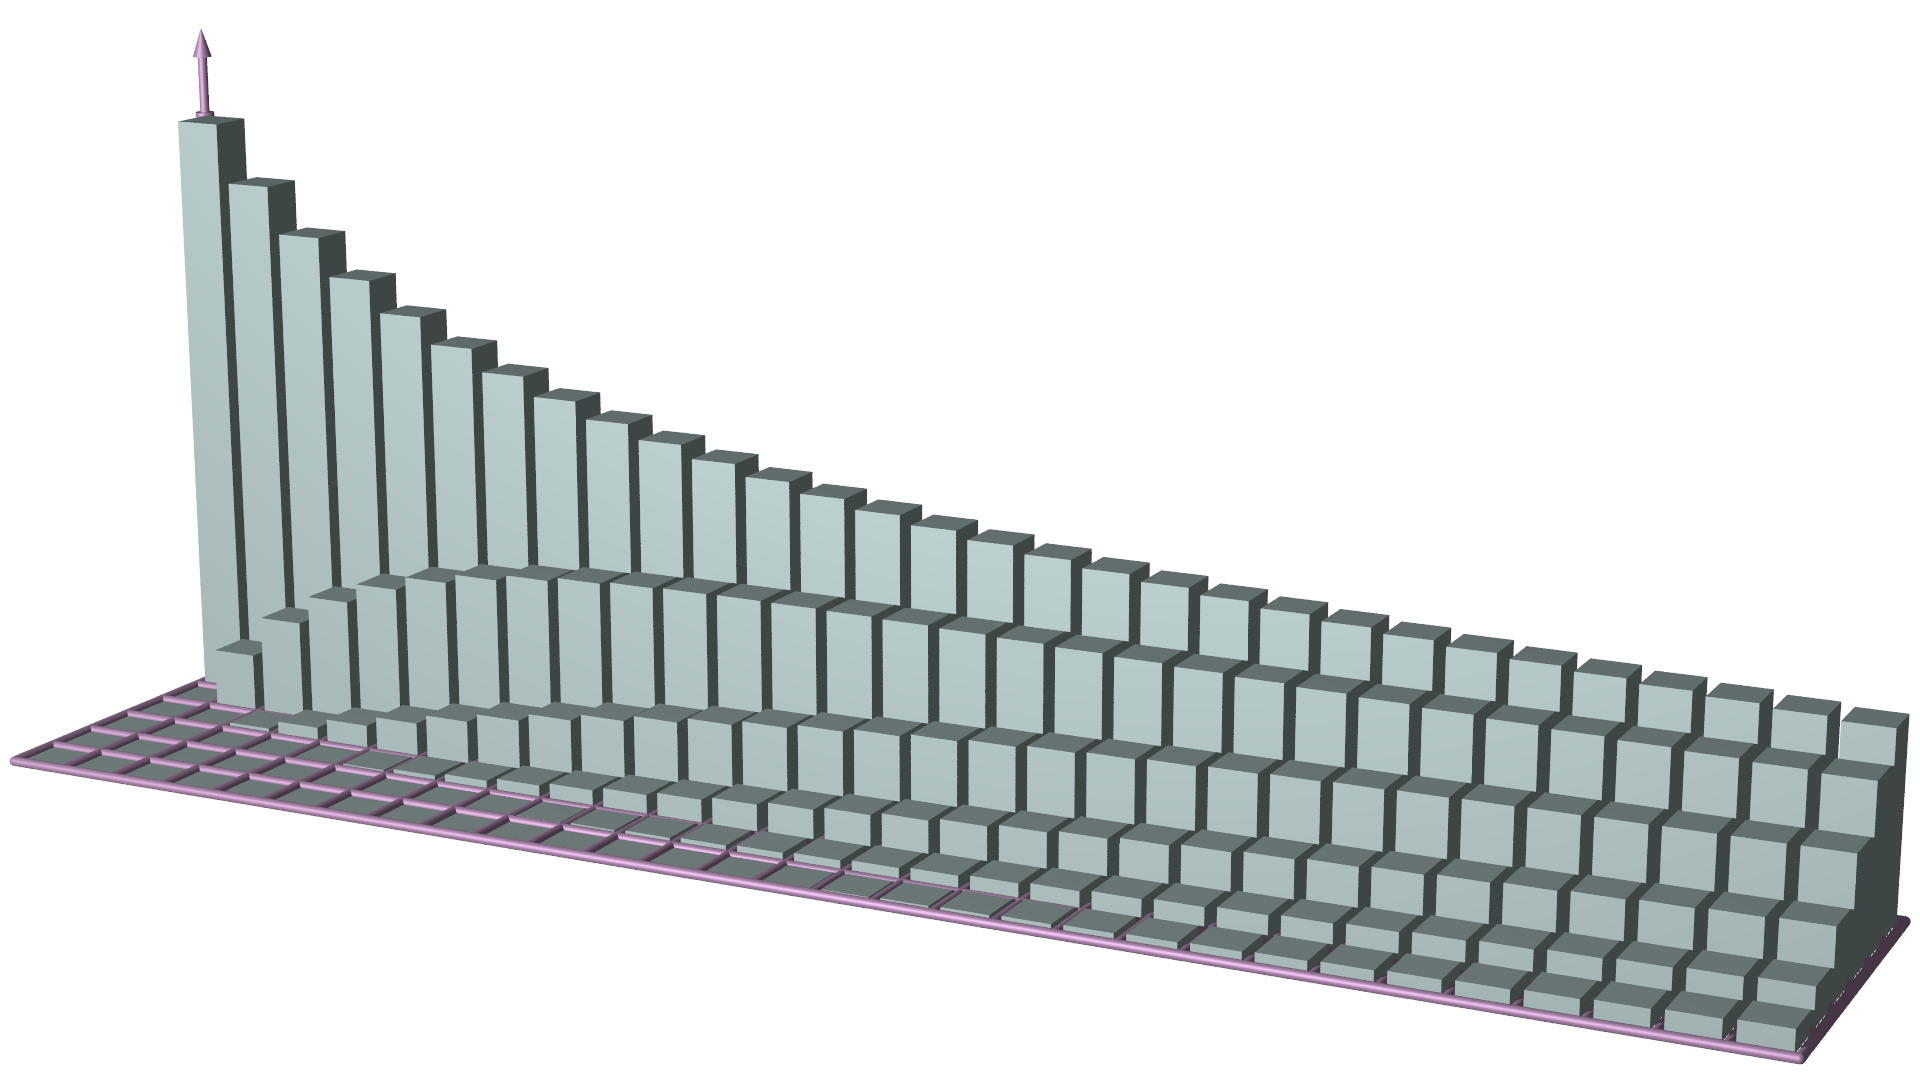
\includegraphics[width=12cm]{diffusion.jpg}};

\node at (-6.3,-1.2) [rotate=-10] {$k=6$};
\node at (-5.15,-0.7) [rotate=-10] {$k=1$};

\node at (5.8,-3.25) [rotate=-10] {$k=6$};
\node at (6.3,-2.5) [rotate=-10] {$k=1$};

\node at (-6.2,-1.7) [rotate=26] {$n=1$};
\node at (4.8,-3.7) [rotate=53] {$n=30$};

%\foreach \x in {-6,-5.9,...,6.01}{
%	\draw[line width=0.1pt] (\x,-3.5) -- (\x,3.5);
%}
%\foreach \x in {-6,...,6}{
%	\draw[line width=0.5pt] (\x,-3.5) -- (\x,3.5);
%	\node at (\x,-3.5) [below] {$\x$};
%}
%\foreach \y in {-3.5,-3.4,...,3.51}{
%	\draw[line width=0.1pt] (-6,\y) -- (6,\y);
%}
%\foreach \y in {-3,...,3}{
%	\draw[line width=0.5pt] (-6,\y) -- (6,\y);
%	\node at (-6,\y) [left] {$\y$};
%}
%\fill (0,0) circle[radius=0.05];

\end{tikzpicture}
\end{document}

